\documentclass{article}
\usepackage[utf8]{inputenc}
\usepackage{amsmath}
\usepackage{mathrsfs}
\usepackage{graphicx}
\usepackage{blindtext}
\usepackage{csquotes}
\usepackage{enumitem}
\setlist[enumerate]{itemsep=0mm}
\usepackage[colorlinks=true,citecolor=blue]{hyperref}
\usepackage[english]{babel}
\usepackage[backend=biber, style=numeric]{biblatex}
\addbibresource{references.bib}

\title{Draft}
%\author{Cheng}
%\date{2018}

\begin{document}
%\maketitle{}
\begin{abstract}
% motivation
% outcome
    The algorithm selection method based on machine learning is widely applied, with the development of such methods that is driven by data and capable of learning how to do for new tasks, those kinds of algorithm can address the problem that need to be told originally by expert to solve certain task, however there still exists a few of work needed to done manually. As such, a novel approach on algorithm selection under the way of deep learning is purposed here, which make use of Convolution Neural Network to automate complicated feature engineering, integrated with gradient descent, the whole procedure from training to predicting can be conducted by one step, it significantly simply the job by human and its performance also get appear enhancement.
\end{abstract}

\section{Introduction}
% context
% need
% task
% structure
    The algorithm selection problem\cite{rice1976algorithm} is concerned with selecting the best algorithm to solve a given problem instance on a case-by-case basis. It has become especially relevant in the last decade, with researchers increasingly investigating how to identify the most suitable existing algorithm for solving a problem instance instead of developing new algorithms\cite{kotthoff2016algorithm}.
    
    Algorithm selection has become gradually more significant as the basic heuristic algorithm is getting huge growth for some particular problems. For instance, while we encounter a group of certain deterministic problem, all of them can not be solved completely using just one algorithm continuously, thus it can point one algorithm for one problem with the help of algorithm selection, especially the problem with expensive computation, much cost would save. Vast problems such as Graph coloring problem\cite{leighton1979graph,galinier1999hybrid},Combinatorial Search problem\cite{kotthoff2016algorithm} and Constraint satisfaction problem\cite{smith2009cross} have be addressed by algorithm selection.
    
    With the wide application of algorithm selection, much more convenient model function involving building, training and predicting is in the status of massive demand, though more excellent machine learning method is emerging continually, such methods make it possible that decision process can be learned alone from existing data rather than domain knowledge summarized by human expert, however there still exists complicated part to deal manually, but they have limited effect on the efficiency enhancement. The fact that feature extraction and based it, suitable model method need to selected for predicting which heuristic algorithm should be used towards a given problem instance still puzzle lots of people in research and product. Massive experiences not only are required, but also too much time and patients.
    
    To improve the experience of solving such problem quickly, efficiently and simply, we thought whether the procedure of extracting features and determining the model can be done easily, even automatically, as such, we studied the deep learning\cite{lecun2015deep} and introduced convolution neural network\cite{krizhevsky2012imagenet} model to address such problems.
    
    This article described a idea of the algorithm selection model with convolution neural network. Relative background in detail and elaborated methodology are provided in section 2 and 3, respectively. Section 4 represented the experiment procedure and section 5 summarize the experiment, as well as follow-up work.

\section{Background}
% context in detail
% introduce cnn
    The primitive algorithm selection problem was proposed by Rice\cite{rice1976algorithm}, it is a simple idea that there is two mapping, shown as formula[\ref{fml:selection-map}], one is a selection mapping $S$ from problem space $\mathcal{P}$ to algorithm space $\mathcal{A}$, and others $P$ map the combination $(x,a)$ to performance measure space $\mathcal{R}^n$, lastly a precise performance result would come out calculated by norm operation, that is the algorithm performance.
    \begin{equation}\label{fml:selection-map}
    \begin{split}
    x &\stackrel{S}{\longrightarrow}a\;\;\;\;a\in\mathcal{A},x\in\mathcal{P} \\
    x,a &\stackrel{P}{\longrightarrow}p\;\;\;\;p\in\mathcal{R}^n \\
    ||p|| &\in\mathcal{R}
    \end{split}
    \end{equation}
    the $||p||$ would be a evidence to determine which decision is good or bad. Consequently, it is algorithm mapping $S$ and measure mapping $P$ that is vital point for better $p$.
    
    The evidence of algorithm mapping is the feature of problem, which is a few explicit or implicit characteristic of problem instance, intuitively speaking, every problem instance can be recognized well by such feature in the best situation, there is however no such situation almost, so in most cases extracting effective feature would be complicated work and whether you deal with the job well is critical for final determinations.
    
    Machine learning technique currently has became the major method to do decision in the past several decades with the evolution of various data-driven method. Therefore, some change has happened in the whole selection model, the selection mapping $S$ is not defined by human experience but data completely, which make it possible that better decision can be conducted efficiently and automatically.
    
    The single algorithm is typically selected by the selection model to solve a given problem, later an algorithm schedule is also defined by the similar model. As for any unique problem instance, there is one unique relative algorithm as long as they have different features, it is hard to get such perfect feature representation and to solve every problem well with just one algorithm, as soon as the wrong decision is made, the whole task would get bad performance. Algorithm schedule therefore is required, which is a list of algorithm that has certain fixed ordering and time slice. Finding multiple algorithms and running it in a certain order and in a way that all of them have a specified slice of time is its core ideas, which can confirm that the worst results would not emerge. In this article, the selection of single solver is main option.
    
    According to those mentioned above, great features must result in better single algorithm. While the feature extraction is big and complicated task, is it possible to automate this process? Of course, deep learning is such a technique that integrate feature extraction and model selection together. Deep learning is getting more and more popular in many research areas and in practice it is indeed applied widely in all kinds of productive task in the past decades. Deep learning further represent a thought that the structure between input and output of the model is a network, in which basic element is a 'neuron' like nerve cell from biology and special function from mathematic, and particular information are transfered within all of neurons in a way that a group of neurons, that is called layer, connect other groups one by one. 
    
    Convolution neural network is determined within vast deep learning structure here, it has excellent ability of handling 2-dimension data such as image. Convolution neural network chiefly consists of convolution operation, pooling operation and forward-net. Convolution operation is employed to extract features automatically by sliding a box named kernel on the image orderly and completely, and what we do is to initialize all of the parameters, including kernel and bias, which is a matrix and scalar respectively. These parameters would update by stochastic gradient descent and back-propagation as the training process is conducting. Pooling operation have two main effect, one is reduce the size of 2-dimension instance by counting the feature of previous step, others is capable of confirm the shift invariance of data like image. Forward-net is used to do the final decision. 
    
    %when to create portfolio
    %when to select

\section{Methodology}
% sufficient detail to reproduce the experiments
    In the basis of deep learning technique, convolution neural network(CNN) primarily used here, the most complicated work of such algorithm selection problem, feature engineering, is completely solved by its advantage of CNN, and the performance of model have vast advance with the help of excellent training method on deep learning.
    
    Format conversion is essential for the convolution neural network. The input of CNN is image format, while the problem instance is saved in the format of text, certain conversion method is required. The most character of instance text is digit, some comment is unimportant and can be ignored. As for all of the characters except comment and definition command, they can be converted to ASCII code, for example,
    \begin{enumerate}[itemsep=-1mm]
        \item c A permuted SAT Competition 2007 formula with seed=1885152118
        \item p cnf 140 560
        \item -65 71 113 -63 0
        \item -4 97 134 -136 0
        \item 10 105 -92 -84 0
    \end{enumerate}
    list above is a snippet of source text file, line 1 show comment about this instance, and line 2 define some information, the rest of line is the main file about this instance. The sequence '$45\ 54\ 53\ 32\ 55\ 49\ 32\ 49\ 49\ 51\ 32\ 45\ 54\ 51\ 10$' is converted from line 3.
    In addition, in order to save memory in the process of computing, some successive character located in the end of line, i.e. '$...63\  0\backslash{n}$', is meaningless and could be ignored except newline sign.
    
    Our CNN model start with three convolution layer, then three full-connected layer, shown as figure[\ref{fig:CNN architecture}], in which last layer is a softmax layer and represent the last selection result in a way that its value is the probable probability of every solver for a given problem instance, if bigger the values is and more feasible the corresponding solver could be, therefore there must be a highest value from this layer and it would be the solution of given problem in most cases. The input size of CNN is $128\times 128$, that is not absolute and other size can be utilized based on the detailed case; the dropout\cite{krizhevsky2012imagenet} layer is introduced into the CNN after pooling layer and it would take effect greatly in the work of preventing CNN from overfitting in a way of randomly dropping units along with their connections from the neural network during training.
    
    \begin{figure}[htbp!]
        \centering
        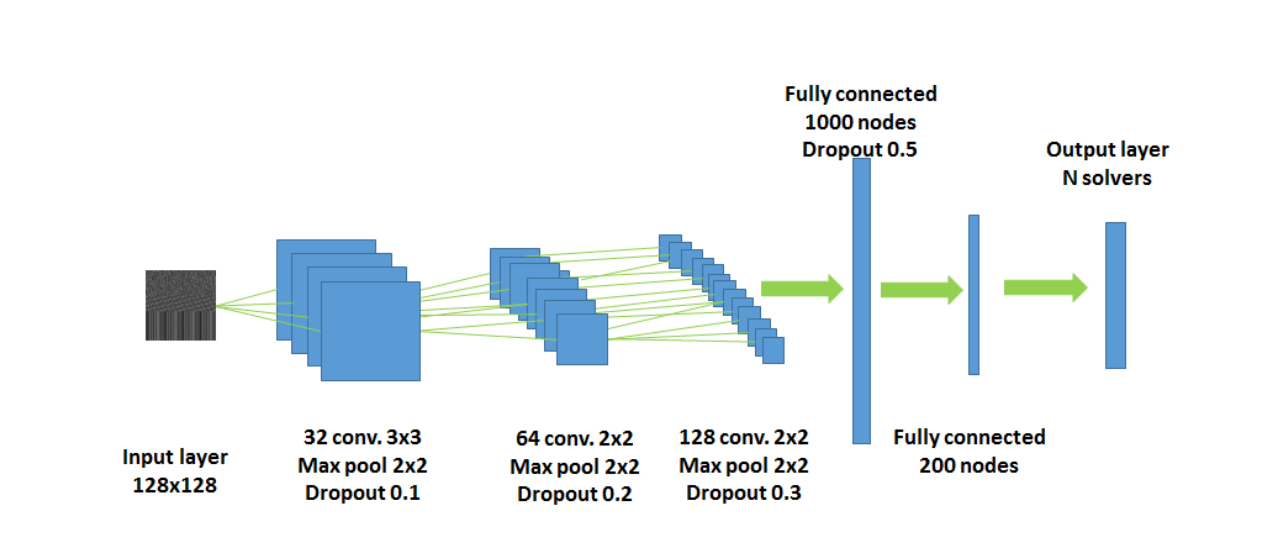
\includegraphics[scale=0.3]{./assets/cnn-ap.png}
        \caption{Elaborated architecture of CNN model}
        \label{fig:CNN architecture}
    \end{figure}
    
    The training method we used is stochastic gradient descent !!!%TODO cite
    during the process of training, Nesterov momentum !!!%TODO cite
    technique is employed to facilitate the speed of training. When the training data is used to fit the network model and thought of validity and cost, batch training is employed and the mini-batch is setting to $64$, learning rate and momentum begin with 0.3 and 0.9, both of them are dynamic to confirm the speed and accuracy of model, and would decrease to 0.001 and 0.999, respectively. The non-linear activation function is the rectify function $\Phi(x) = max(0, x)$, but the activation function of softmax layer, is setting to sigmoid function $\Phi(x) = \frac{1}{1+e^{-x}}$. The output of network actually is a column vector consisting of multiple predicted value $p$, its length is the number of the solver and any value $p$ of them denote the probability that this corresponding solver can address a given problem. The binary log loss function $L = -y \log(p)-(1-t)\log(1-p)$ is to gauge the difference between the real and the predicted, in which $y\in {0,1}$ denote the real label of the solver, and $p \in [0,1]$ denote the predicted value.
    
    There are three evaluation method to test whether the performance of predicted solver for the problem instance at hands is excellent or not. PAR10 scores is a measurement of the time required to run on all problem instances, if an instance was solved within the timeout by the algorithm the model chose, the actual runtime is taken, and if a timeout occurred, the timeout value was multiplied by $10$. Percentage solved records the percentage of problem instances in the data set for which the model selected an algorithm that was able to solve it with run-status "ok" and the algorithm time plus the feature computation time was at most the timeout. Misclassified solver, given a threshold value towards softmax output, is to record the the number of incorrect selection, including false positive selection, that is the selection which predicted value is bigger than threshold but actual value is $0$, and false negative selection, that is the selection which predicted value is smaller than threshold but actual value is $1$, it can formulate as follow
    \begin{equation}\label{fml:misclassified-solver}
    y^* = \left\{ \begin{array}{rcl}
    1 ,  y \geq threshold \\
    0 ,  y \le threshold
    \end{array}\right.
    \end{equation}
    the threshold in this experiment is set to $0.5$, 1 represent the problem can be solved with this solver and 0 represent the problem can not be solved.

\section{Experiment}
    The experiment environment is in the basis of ubuntu16.04, the framework used is tensorflow1.6, meanwhile accelerating computation with GPU. Image generation rely on Pillow and Numpy package.

    While we start training this model, the data set with distinct scenarios need to prepare. In ASLib\cite{bischl2016aslib} website, which is a website that provides vast scenarios and its authoritative benchmarks to simply the process of comparing different algorithm performance for same data sets, there are a lot of experiment data, note that it is not the data sets of the source problem instance, but the data analogous to instance label information, including all of knowledge of features, available solver, as well as their run time and so on. Our data sets is chiefly SAT problem instance and relative statement or analysis mentioned later are basing on SAT problem instance. For instance, SAT12-HAND data sets, it have 767 instances, 31 algorithms or solvers and 115 features crafted by human.

    SAT scenarios is a common problem sets and many problem can convert to SAT problem with a CNF format, this make it more meaningful that solving SAT problem is acceptable or complete. SAT problem instance are presented with CNF file format, which is the numerical collection of abstract data, like shown above. While we convert the cnf text file, something trivial in cnf file would be ignored, the real meaningful data is numerical characters, as well as the space and newline.  When all of the character have been being in the mode of pure digit, then much so big digit sequence need to become matrix and reduce the shape of matrix. There are several method to handle matrix reduction, here we use % TODO reduction method and final shape

    For better training experience, the data need to be preprocessed by subtracting the mean and normalizing each image with scikit-learn package. Figure[\ref{fig:CNF-image}] show image with conversion from cnf file.

    \begin{figure}[htbp!]
        \centering
        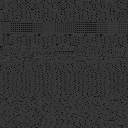
\includegraphics[scale=0.7]{./assets/cnf-image.png}
        \caption{The image after conversion from cnf file}
        \label{fig:CNF-image}
    \end{figure}

    As a comparison of evaluation of model performance, we can find some benchmarks with various selection strategies in ASLib website. Virtual best solver(VBS), which always select the best solver for every problem, is a ideal method that is unable to be surpassed by other method in performance, best single solver(BSS), which is a method of selecting merely single best solver for all problem, is the oldest method to solve a batch of problem, of course, there are some benchmarks dealing with machine learning, like random forest and supported vector machine.
% TODO more benchmark or DLforAP baseline

    % TODO validation: cross or hold-out
    The data sets of every scenarios require to be divided into equal part, its length is 

\subsection{Result}

    \begin{figure}[htbp!]
        \centering
        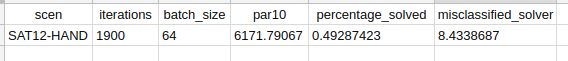
\includegraphics[scale=0.6]{./assets/exp_res.png}
        \caption{The experiment result}
        \label{fig:experiment result}
    \end{figure}

\subsection{Discussion}

\section{Conclusion}

\printbibliography
\end{document}